\chapter{Experiments}

In the experimental phase, we selected datasets that have previously been utilized in well-recognized competitions. This allows us to benchmark the 
performance of our model against established baselines and leading-edge results within the field, helping us make meaningful comparisons with our model. 
Each dataset employed in our experiments represents a common scenario in the field of object detection, encompassing diverse environments and perspective 
urban life captured through ground-level cameras, aerial views provided by drones, and wide-ranging perspectives from satellites. 

\section{Datasets}
For the benchmarking of our model we decided to use three very well known datasets, and we are going to analyze in this section.


\subsection{Microsoft Common Object in COntext (MS COCO)}
The Microsoft Common Objects in Context (MS COCO) dataset 2017 \cite{COCOdataset} is a comprehensive image dataset designed for object detection, segmentation,
and captioning tasks. It is known for its complexity of its images, which are primarily sourced from everyday scenes. The dataset includes 80 object categories, 
providing a wide range of common objects for robust training and evaluation of machine learning models. These categories encompass various items from person, bicycle, 
car, to stop sign and smaller objects like toothbrush.

In terms of its composition, the MS COCO 2017 dataset contains over 118,000 training images, 5,000 validation images, and a test set of around 41,000 images, 
bringing its total to approximately 164,000 images. This dataset is also accompanied by over 1.5 million object instances, each annotated. 
The annotations are formatted to support both object detection and instance segmentation tasks. Specifically, for object detection, each annotation includes 
not only the class label and a bounding box defined by the $x$ and $y$ coordinates of the top-left corner, width, and height, but also a detailed segmentation 
mask for each object instance, making it suitable for more granular segmentation tasks as well.

The dataset is divided into training, validation, and test splits to facilitate the training and fine-tuning of models in a structured manner. 
This split ensures that models can be trained on a large set of images and parameters can be fine-tuned on the validation set before final evaluations 
are performed on the test set. The use of MS COCO for competition and research has helped advance the field of computer vision by providing a challenging 
set of images and annotations that test the limits of both existing and novel visual recognition models.

\newpage

Class Distribution in COCO 2017:

\begin{figure}[h!]
    \centering
    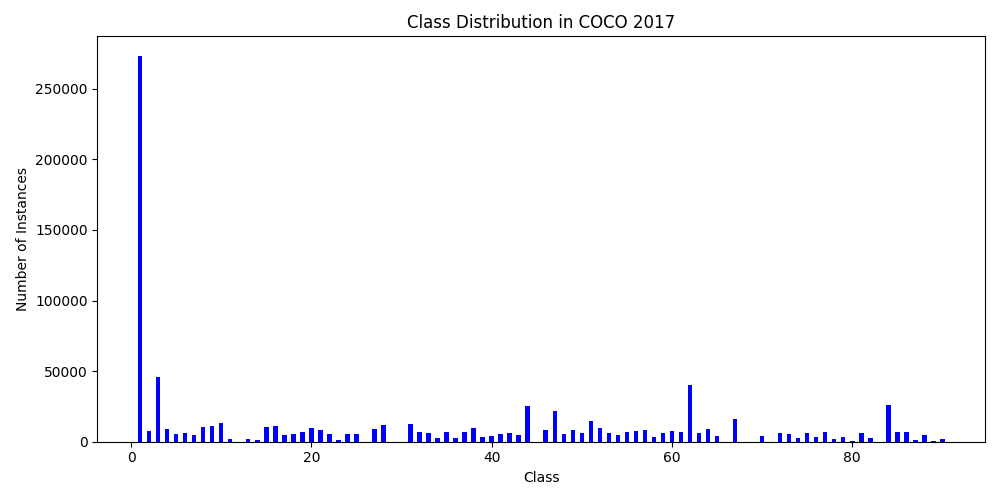
\includegraphics[scale=0.55]{Figures/coco2017_class_distribution.png}
    \caption{Class Distribution in COCO 2017}
    \label{fig:coco-class}
\end{figure}


Calculating the mean and standard deviation of the bounding boxes and masks is crucial for generating more precise anchors, as it allows us to tailor the anchor sizes 
and aspect ratios to the actual distribution of objects in the dataset. This not only improves detection accuracy by aligning the anchors more closely with the objects, 
but also reduces unnecessary complexity by minimizing the need for an excessive number of anchors, which can lead to increased computational cost without performance gains.
With that point in mind we calculated and store the following:

\begin{table}[h]
    \centering
    \begin{tabular}{|c|c|}
        \hline
        Metric                     & Number of Pixel   \\ \hline
        Mean Width                 & 100               \\ \hline
        Mean Height                & 104               \\ \hline
        Width Standard Deviation   & 123               \\ \hline
        Height Standard Deviation  & 111               \\ \hline
    \end{tabular}
    \caption{Basic statistics of COCO dataset bounding boxes}
    \label{tab:coco_bboxes}
\end{table}


\newpage
\subsection{Unmanned Aerial Vehicle Small Object Detection}

The UAV-SOD (Unmanned Aerial Vehicle Small Object Detection)  \cite{UAVSmallObjectKaggle}  dataset is specifically designed for advancing research in the area of object 
detection using aerial imagery captured by drones. This dataset focuses on the detection of small objects, which presents unique challenges due to the small 
scale and often complex backgrounds seen in aerial images. Here are the key details about the UAV-SOD dataset. The UAV-SOD dataset includes detailed annotations 
for each image, essential for supervised machine learning models such as object detectors. Annotations are provided in XML format compatible with the PASCAL VOC 
annotation format, which is widely used in object detection tasks. These annotations include bounding boxes that specify the coordinates of each object in the image. 
The objects in this dataset are annotated with their class labels, enabling not only object detection tasks but also potential use for object classification 
and segmentation challenges.

Class Distribution in UAV Small Object Detection:

\begin{figure}[h!]
    \centering
    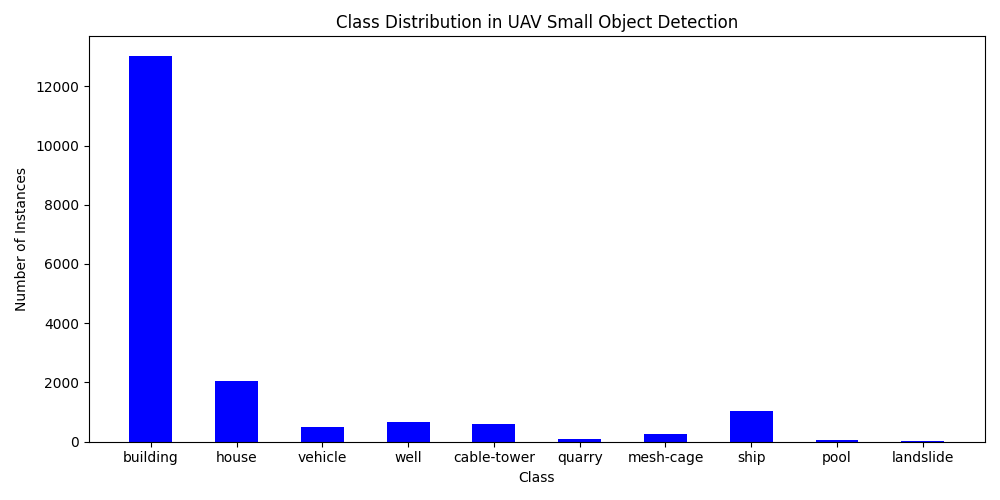
\includegraphics[scale=0.55]{Figures/uav_sod_data_class_distribution.png}
    \caption{Class Distribution in UAV Small Object Detection}
    \label{fig:uav-class}
\end{figure}


Once again computing the mean and standard deviation of the bounding boxes and masks helps ensure that the anchors are appropriately scaled to the objects in the dataset, 
reducing unnecessary complexity in the model.
\begin{table}[h]
    \centering
    \begin{tabular}{|c|c|}
        \hline
        Metric                     & Number of Pixel   \\ \hline
        Mean Width                 & 19                \\ \hline
        Mean Height                & 19                \\ \hline
        Width Standard Deviation   & 16                \\ \hline
        Height Standard Deviation  & 17                \\ \hline
    \end{tabular}
    \caption{Basic statistics of UAV-SOD dataset bounding boxes}
    \label{tab:uav_bboxes}
\end{table}

\newpage
\subsection{VisDrone}

VisDrone \cite{VisDroneDataset} is a dataset designed for drone-based object detection, featuring $10,209$ images captured across various environments using different 
types of drones. Each image in the dataset has a high resolution of $2000 \times 1500$ pixels. The dataset is organized into splits for comprehensive 
training and evaluation, consisting of $6,471$ images for training, $548$ images for validation, and $3,190$ images for testing. VisDrone includes a 
diverse set of ten object classes, such as pedestrians, cars, vans, buses, trucks, motorcycles, bicycles, awning-tricycles, and tricycles. This wide 
range of categories, combined with the diverse aerial perspectives provided by drone capture, makes VisDrone an ideal resource for developing and 
benchmarking deep learning models focused on enhancing object detection capabilities in drone surveillance systems.

Class Distribution in VIS Drone:

\begin{figure}[h!]
    \centering
    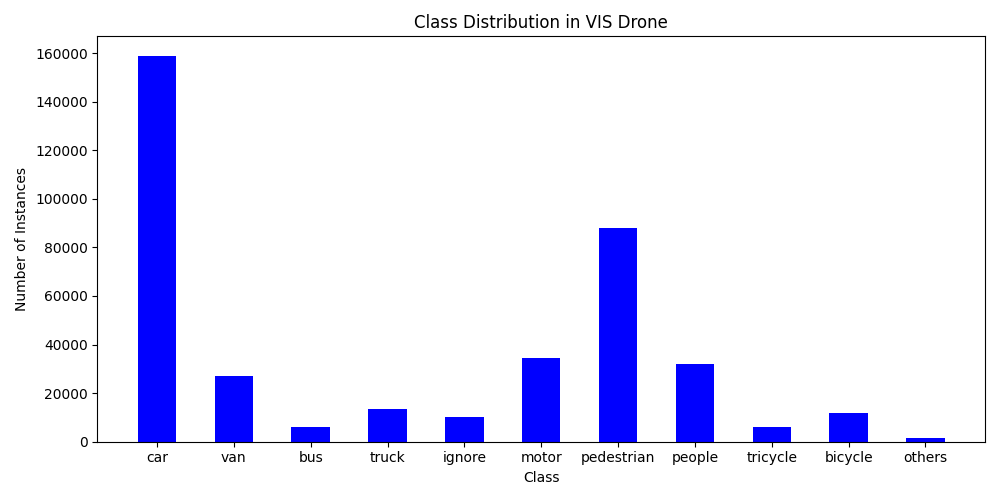
\includegraphics[scale=0.55]{Figures/vis_drone_data_class_distribution.png}
    \caption{Class Distribution in VIS Drone }
    \label{fig:vis-class}
\end{figure}

By determining the mean and standard deviation of the bounding boxes and masks, we optimize the anchor generation process, leading to more efficient object detection 
without adding unnecessary complexity. These variations convey the same core idea but in a more concise manner, assuming the main explanation has already been 
provided for the first dataset.

\begin{table}[h]
    \centering
    \begin{tabular}{|c|c|}
        \hline
        Metric                     & Number of Pixel   \\ \hline
        Mean Width                 & 15                \\ \hline
        Mean Height                & 14                \\ \hline
        Width Standard Deviation   & 16                \\ \hline
        Height Standard Deviation  & 13                \\ \hline
    \end{tabular}
    \caption{Basic statistics of VisDrone dataset bounding boxes}
    \label{tab:vis_bboxes}
\end{table}


\newpage
From what we can detect in the class distributions, a significant class imbalance is present in the datasets. Class imbalance poses a 
challenge in training because models trained on such data may develop a bias towards more common classes and perform poorly on rare classes. 
We have to take this into consideration when choosing the evaluation metrics that give a more nuanced view of class-specific performance, such as 
per-class accuracy, are crucial for assessing a model’s true effectiveness across the varied classes present in these datasets.
Finally the COCO 2017 dataset is commonly used as a benchmark in object detection tasks, though it is not specifically designed for small object detection. 
The mean and standard deviation of its bounding box sizes indicate that it includes a wider range of object sizes, with many larger objects. While the COCO dataset 
is useful for evaluating general object detection performance, datasets like UAV-SOD and VisDrone are more focused on small object detection, as reflected in 
their much smaller average bounding box sizes, making them more appropriate for detecting smaller objects in complex environments.

\newpage
\section{Data Pre-Processing}

To ensure that the object detection models are trained on well-structured and uniform data, pre-processing steps are applied to standardize and enhance the 
raw dataset inputs. This process is crucial for achieving optimal model performance and is applied consistently across different datasets, such as COCO2017, 
UAV-SOD Drone, and Vis-Drone datasets, with specific adjustments tailored to each dataset's unique characteristics.

Firstly we have some general pre-processing steps applied across all datasets in order to make the training procedure 

\begin{enumerate}
    \item Resizing Images and Annotations: All images and corresponding annotations are resized to a uniform size of \(600 \times 600\) pixels. 
    This standardization helps maintain consistency across the dataset, which is crucial for the feature map creation with the Efficient-B7 model. 
    The resizing function also handles the segmentation data associated with each image, ensuring that all spatial information (bounding boxes and 
    segmentation masks) is correctly scaled and translated according to the new image dimensions.

    \item Image Padding: To maintain aspect ratio without distorting the image content, padding is applied using the most common color found in the image. 
    This approach prevents the introduction of biases that could occur if a non-representative color was used.

    \item Annotation Format: The annotation files for all the datasets have a common format in order to avoid any problems with the training process. The format 
    is the following: $x_{min}, y_{min}, x_{max}, y_{max}$, class code, $[(x_1, y_1), (x_2, y_2), ..., (x_n, y_n)]$, where the first four 
    values are the bounding box coordinates following the Pascal VOC format, then we have class code of the object and lastly the 
    list of coordinates describing the mask of the object.

    \item Mask Creation: The masks are a vital part of the model, since we want to use the functionality of the Masked-Attention Mask Transformer 
    in combination with the bounding box functionality to get better and more detailed results. The datasets ViS-Drone and 
    Unmanned Aerial Vehicle datasets do not include masks and in order to have mask data we generate masks from the bounding box 
    data. More specifically the mask data format is the following: \\
    $[(x_{min}, y_{min}), (x_{min}, y_{max}), (x_{max}, y_{min}), (x_{max}, y_{max})]$

    \item Calculation of Mean and Standard Deviation: For normalization purposes, the mean and standard deviation of the pixel values across the dataset are 
    computed. These statistics are essential for normalizing the images during the model training process, 
    allowing for faster convergence and improved generalization.

    \item Visualization of Data: Functions are included to plot images alongside their annotations for both training and validation sets. This visual check 
    allows for the verification of the correct processing and annotation of the data, ensuring integrity before training begins.

  \end{enumerate}



\newpage

Furthermore we make specific changes to each dataset in order to ensure compatibility with the model. These changes are:

\begin{enumerate}
    \item \textbf{COCO2017 Dataset - } Annotation Conversion: The original COCO annotations are converted into a simpler text format that includes bounding 
    box coordinates and segmentation data. This conversion facilitates the use of custom training pipelines that may not natively support COCO's complex 
    annotation format.

    \item \textbf{Vis-Drone Dataset - } Annotation Format Standardization: The annotations provided with the Vis-Drone dataset are standardized to ensure 
    consistency with other datasets. This process includes recalculating bounding box coordinates from $[x_{min}, y_{min}, width, height]$ to  
    $[(x_{min}, y_{min}), (x_{min}, y_{max}), (x_{max}, y_{min}), (x_{max}, y_{max})]$

    \item \textbf{UAV-SOD Drone Dataset - } XML to Text Conversion: Given that UAV-SOD annotations might be provided in XML format, a conversion process 
    is implemented to translate these XML files into a plain text format that is easier to manipulate and integrate into training workflows. The conversion 
    also involves mapping categorical names to predefined numerical codes, which are crucial for consistent label encoding across different datasets.
\end{enumerate}

These pre-processing steps are critical for preparing the data, ensuring that it meets the necessary format and quality standards required for effective 
model training. This comprehensive approach to data preparation helps in minimizing issues during training, leading to more robust and accurate object 
detection models.



\section{Evaluation Metrics}


Evaluation metrics are vital in object detection as they quantitatively measure a model's accuracy, robustness, and effectiveness in predicting correct 
object locations and classifications. These metrics enable developers to compare different models, optimize parameters, and ensure that the system performs 
well across various conditions and datasets, guiding improvements and ensuring that the deployed models meet the required performance standards. Starting 
with the basic definitions we have:

\begin{enumerate}
    \item True Positives (TP) \cite{metrics} are the predictions that correctly match the class of the ground truth AND Confidence and IoU scores are 
    higher than their thresholds.
    \item False Positive (FP) \cite{metrics} are the predictions that incorrectly predict a positive class when the ground truth is actually negative 
    OR the IoU score is lower than the threshold.
    \item False Negative (FN) \cite{metrics} occurs when the model misses positive instances. It predicts a negative class when the ground truth is actually positive.
    \item True Negative (TN) \cite{metrics} represents instances where the confidence score of a detection that is not supposed to detect anything is lower than 
    the threshold. This metric is not used in the object detection field since there are too many boxes that should not detect an object in an image.
\end{enumerate}


The metrics we are going to be using that are object detection specific are the Average Precision (AP), mean Average Precision (mAP), Intersection over 
Union (IoU), Average Recall (AR) and mean Average Recall (mAR). \\


Recall \cite{metrics} measures the proportion of actual positives that are correctly identified by the model, indicating the model’s ability to detect all relevant instances.
\begin{equation}
    \text{Recall} = \frac{TP}{TP + FN} \tag{16}
\end{equation}


Precision \cite{metrics} indicates the accuracy of the positive predictions made by the model, measuring the proportion of positive identifications that were actually correct.
\begin{equation}
    \text{Precision} = \frac{TP}{TP + FP} \tag{17}
\end{equation}

F1-Score \cite{metrics} is the harmonic mean of precision and recall, providing a balance between the two by penalizing extreme values.

\begin{equation}
    F1 = 2 \cdot \frac{\text{Precision} \times \text{Recall}}{\text{Precision} + \text{Recall}} \tag{18}
\end{equation}


Intersection Over Union (IoU) \cite{metrics} assesses the overlap between predicted bounding boxes and ground truth boxes, quantifying the exactness of the location 
of predictions. It is a fundamental metric for determining whether a detection is a true.

\begin{equation}
    IoU = \frac{\text{Area of Overlap}}{\text{Area of Union}} \tag{19}
\end{equation}


Average Precision (AP) \cite{metrics} quantifies the precision of an object detector across different recall levels by taking the mean of precisions computed 
at the point of each of the 11 recall levels. The precision at each recall level $r$ is interpolated by taking the maximum precision measured 
for a method at any recall level $\geqslant r$

\begin{equation}
    AP = \frac{1}{11} \sum_{r \in \{0.0, 0.1, \ldots, 1.0\}} P_{\text{interp}}(r) \tag{20}
\end{equation}


Mean Average Precision (mAP) \cite{metrics} is the average of the AP scores for all classes or over different Intersection over Union (IoU) thresholds. 
This metric gives an overall effectiveness of the detection model across various object categories or detection precisions, making it ideal for 
scenarios where multiple object types are involved.
\begin{equation}
    mAP = \frac{1}{N} \sum_{i=1}^{N} AP_i \tag{21}
\end{equation}


\newpage
\section{Training}

To implement the Extended Masked-Attention Mask Transformer, we utilized Amazon Web Services (AWS) SageMaker for efficient training and experimentation. 
Specifically, we employed the \textit{ml.p4d.24xlarge} instance type for our notebook environment, which is equipped with eight NVIDIA A100 GPUs and supports CUDA 12.1. 
This powerful computational setup allowed us to run the training with a batch size of four images per batch, achieving an optimal balance between convergence 
speed and model accuracy.

The weights of the network were initialized using the default settings provided by PyTorch, ensuring standard initialization practices. All experiments were 
conducted using this configuration to maintain consistency and reliability in our results. By leveraging the capabilities of AWS SageMaker and the high-performance 
computing resources of the \textit{ml.p4d.24xlarge} instance, we were able to efficiently train the model and effectively utilize the limited data from small objects in images.

To provide clarity on our training setup and ensure reproducibility, the table \ref{tab:training_parameters} summarizes the key training parameters used for the 
Extended Masked-Attention Mask Transformer. These parameters were carefully selected based on extensive experimentation to achieve an optimal balance between 
convergence speed and model accuracy.
\begin{table}[h]
\centering
\begin{tabular}{|c|c|c|c|}
    \hline
    &                   \textbf{MS COCO}      & \textbf{UAV-SOD}     & \textbf{VisDrone}            \\ \hline
    Number of Epochs   & 125                  & 75                   & 75                           \\ \hline
    Optimizer          & AdamW                & AdamW                & AdamW                        \\ \hline
    Learning Rate      & $1 \times 10^{-4}$   & $1 \times 10^{-3}$   & $1 \times 10^{-3}$           \\ \hline
    Batch size         & 4                    &  4                   & 4                            \\ \hline
    Image size         & $600\times600$       &  $600\times600$      & $600\times600$               \\ \hline
    Number of Anchors  & $30000$              &  $722$               & $722$                        \\ \hline
\end{tabular}
\caption{Details of training parameters per dataset}
\label{tab:training_parameters}
\end{table}



\newpage

\section{Results}

Following the comprehensive description of our training setup and parameters, we now present the results of our experiments with the Extended Masked-Attention 
Mask Transformer. This section delves into the performance metrics achieved by the model, highlighting its effectiveness in both object detection and instance 
segmentation tasks. We evaluate the model's ability to accurately detect and segment objects of various sizes within images, with a particular focus on its 
performance on small objects, which pose significant challenges due to their limited visual information. For brevity and clarity, we will use the following 
abbreviations throughout:

\begin{itemize}
    \item Masked-Attention Mask Transformer will be referred to as MAMT.
    \item Extended Masked-Attention Mask Transformer will be referred to as EMAMT.
\end{itemize}


The Mask2Former model has a Sliding Window (Swin-L) \cite{swin} backbone, pre-trained on the ImageNet-22K dataset, is the best performing model from the proposed 
Mask2Former variations that we will compare our model against. It operates with 200 queries and was trained for 100 epochs utilizing a total of 216 million parameters. 
This model is computationally intensive, requiring 868 gigaflops (FLOPS) and running at a speed of 4 frames per second (FPS). The use of a pre-trained 
Swin-L backbone adds significant power to its feature extraction, but the high number of parameters and FLOPS highlight the overall complexity and 
computational weight of the model, which can impact efficiency in high-performance tasks.

\subsection{Microsoft Common Object in COntext (MS COCO)}

As expected, the proposed methodology is significantly lighter than original Masked-Attention Mask Transformer, where our model is 56\% lighter in terms of 
number of trainable parameters. This complexity reduction comes at a performance drop of around 6.5\%, which is sensible given the great difference in parameters
and complexity. We can see the performance of each model on the table \ref{tab:coco_results} along with the mAP across IoU thresholds ranging from 0.5 to 0.95.

\begin{table}[h]
    \centering
    \begin{tabular}{|c|c|c|c|c|c|}
        \hline
        \textbf{Model}     & \textbf{mAP(@0.5)}     & \textbf{mAP(@0.5:0.95)}    & \textbf{Queries}   & \textbf{Parameters} & \textbf{GFLOPs}  \\ \hline
        EMAMT              & 44.5                   & 30.2                       & \textbf{100}       & \textbf{95M}        &  \textbf{492}     \\ \hline
        MAMT               & \textbf{50.2}          & \textbf{38.8}              & 200                & 216M                &  868              \\ \hline
    \end{tabular}
    \caption{Results for COCO dataset}
    \label{tab:coco_results}
\end{table}


On the plot seen on the Figrue  \ref{fig:coco-train}, both models demonstrate a rapid increase in mAP during the first 20 epochs, reflecting quick initial learning. 
Afterward, the mAP increases more gradually, indicating that the models are nearing convergence. The MAMT model consistently outperforms EMAMT in both metrics, 
achieving a higher final mAP. The mAP@0.5 performance of MAMT plateaus at around 50\%, while EMAMT stabilizes at 41.5\%. Similarly, for mAP@0.5:0.95, MAMT reaches 
approximately 39\%, while EMAMT stabilizes around 30\%.

These results highlight the trade-off between model complexity and performance. While EMAMT is a lighter model with fewer parameters, it shows a lower 
overall performance compared to MAMT, which has a larger parameter count and FLOPs.

\begin{figure}[h!]
    \centering
    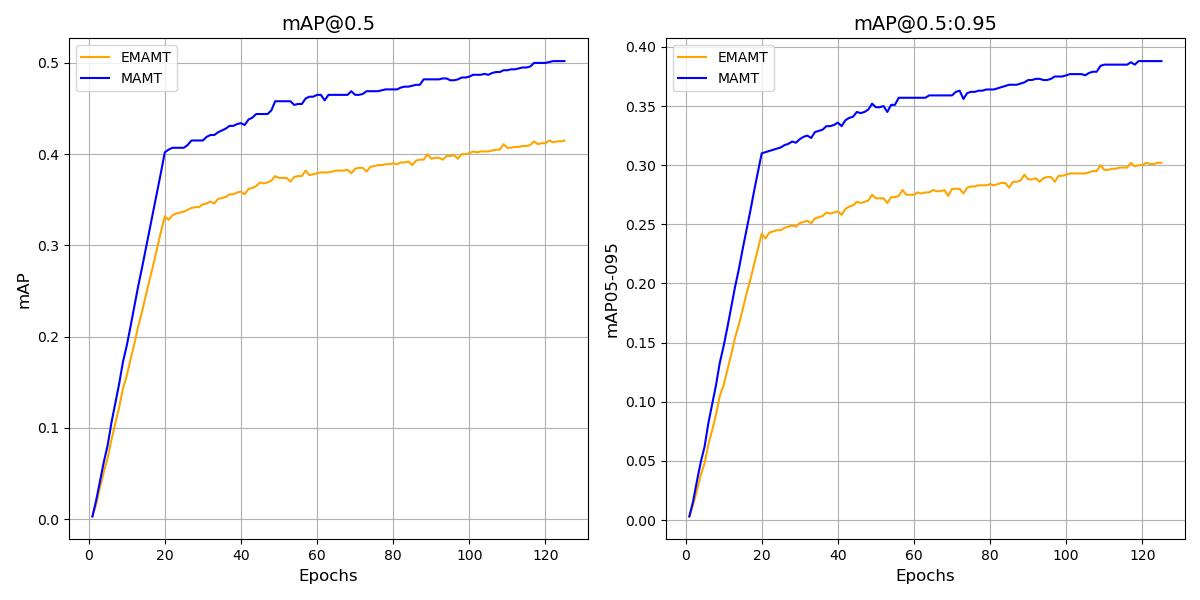
\includegraphics[scale=0.45]{Figures/coco_train.jpg}
    \caption{Performance comparison of MAMT and EMAMT on mAP at 50\% IoU threshold (left) and the average mAP across IoU thresholds from 50\% to 95\% (right) 
    for the COCO2017 dataset}
    \label{fig:coco-train}
\end{figure}


As depicted in Figure \ref{fig:coco-images}, the model successfully detected all the labelled objects. Despite having a lower mAP, the model was able to find the objects with
great precision with the bounding boxes predictions of the EFPN module and a very respectable accuracy by the masks created by the Mask2Former module of the 
EMAMT. It is important to note, that the COCO2017 dataset had a big class imbalance and from what we can see in the Figure \ref{fig:coco-images}, the masks and the subsequent 
bounding boxes from those masks are not as detailed for the objects like the airplanes as the person objects. This difference is to be expected based on the 
class distribution, but we can clearly see that the mask and the created bounding box is accurate enough. 

\begin{figure}[!h]
    \captionsetup{justification=centering}
    \centering
    \begin{minipage}{0.4\textwidth}
      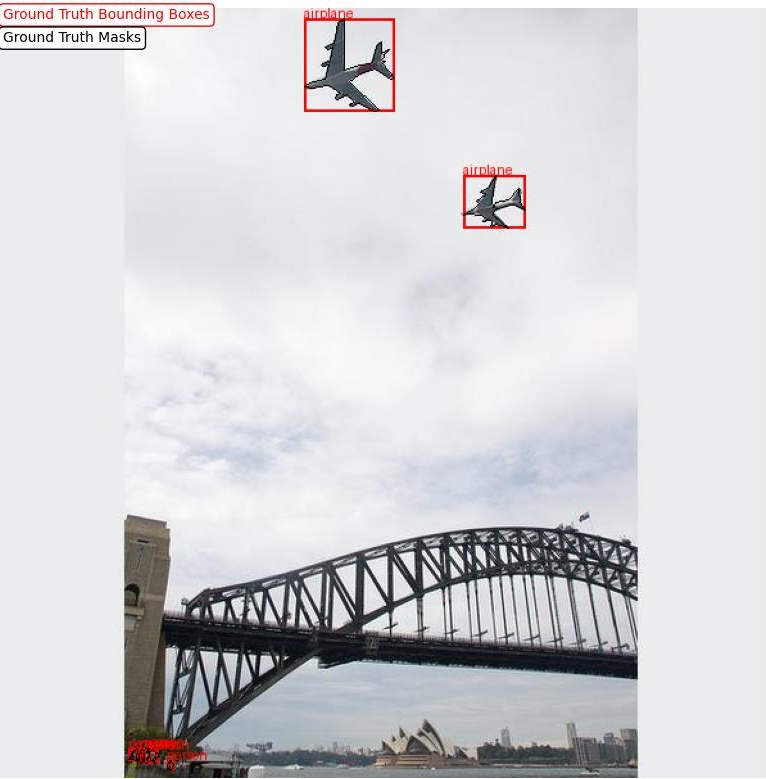
\includegraphics[scale=0.35]{Figures/coco_ground_truth.jpg}
      \caption{Ground Truth Bounding boxes and Masks}
    \end{minipage}
    \hfill
    \begin{minipage}{0.4\textwidth}
      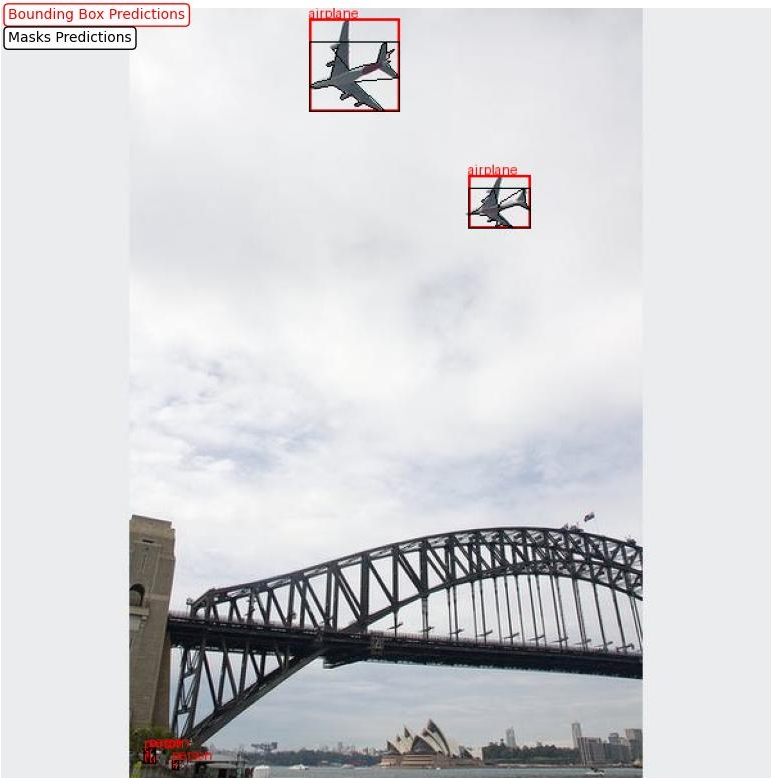
\includegraphics[scale=0.35]{Figures/coco_predictions.jpg}
      \caption{Predicted Bounding boxes and Masks}
    \end{minipage}
    \caption{Comparison between ground truth and predictions of EMAMT for the COCO2017 dataset}
    \label{fig:coco-images}
\end{figure}


\subsection{Unmanned Aerial Vehicle Small Object Detection}

As seen with the COCO dataset, the proposed methodology is substantially lighter. In the UAV-SOD dataset, this reduction in complexity results in a slight 
performance improvement, with the EMAMT model outperforming MAMT by a margin of 3.1\% in mAP(@0.5) and 3.1\% in mAP(@0.5:0.95). This result is particularly 
notable given the significant reduction in both parameters and FLOPs. The detailed results of the two models can be seen in Table \ref{tab:uav_results}, 
showing that our lighter model maintains strong performance even in small object detection tasks.


\begin{table}[h]
    \centering
    \begin{tabular}{|c|c|c|c|c|c|}
        \hline
        \textbf{Model}     & \textbf{mAP(@0.5)}    & \textbf{mAP(@0.5:0.95)}    & \textbf{Queries}   & \textbf{Parameters} & \textbf{GFLOPs}  \\ \hline
        EMAMT              & \textbf{51.3}         & \textbf{39.2}              & \textbf{100}       & \textbf{95M}        &  \textbf{492}     \\ \hline
        MAMT               & 48.2                  & 36.1                       & 200                & 216M                &  868              \\ \hline
    \end{tabular}
    \caption{Results for UAV-SOD dataset}
    \label{tab:uav_results}
\end{table}

Once again both models exhibit a sharp rise in mAP during the first 20 epochs as presented , which signifies efficient early learning. After this initial phase, the 
EMAMT model maintains a higher mAP throughout the training period compared to MAMT, indicating better performance in this dataset. The EMAMT model peaks 
at an mAP@0.5 of approximately 51\%, while MAMT reaches around 48\%. Similarly, for mAP@0.5:0.95, EMAMT stabilizes at around 39\%, outperforming MAMT, 
which plateaus at 36\%.

These results suggest that EMAMT, despite having fewer parameters, manages to deliver superior performance on small object detection tasks, such as in 
UAV-SOD, compared to the larger MAMT model. This highlights the potential of more efficient models to perform well in specialized scenarios where smaller 
objects dominate the dataset.

\begin{figure}[h!]
    \centering
    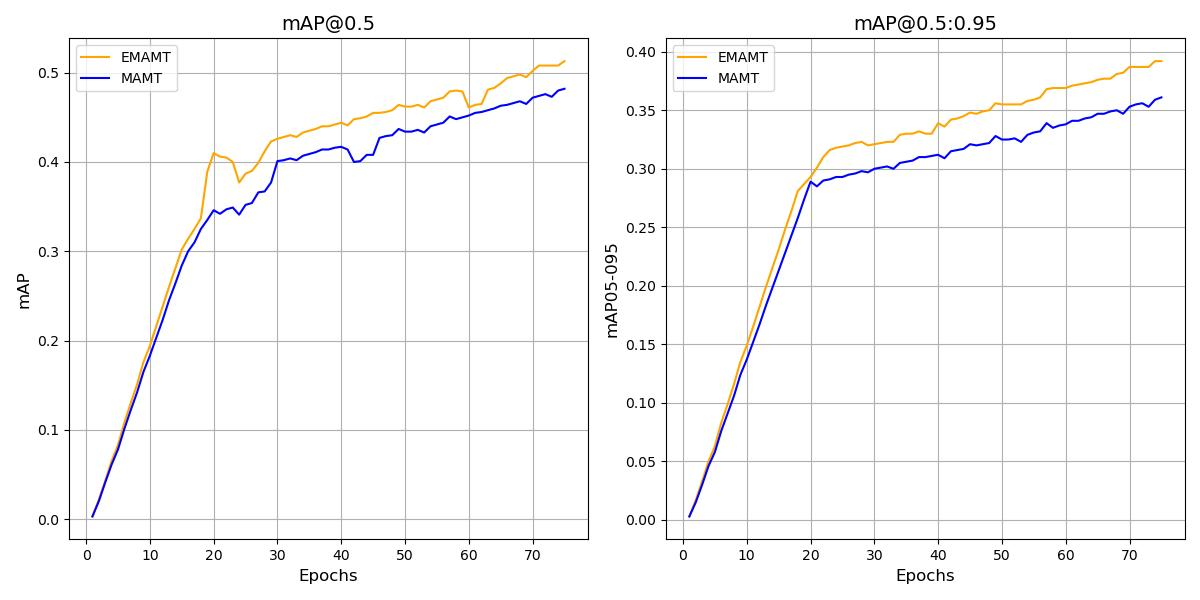
\includegraphics[scale=0.45]{Figures/uav_train.jpg}
    \caption{Performance comparison of MAMT and EMAMT on mAP at 50\% IoU threshold (left) and the average mAP across IoU thresholds from 50\% to 95\% (right) 
    for the UAV-SOD dataset}
    \label{fig:uav-train}
\end{figure}



As depicted in Figure \ref{fig:uav-images}, the model successfully detected all but one of the labelled objects. In this dataset the EMAMT model achieved the best 
results eclipsing the original MAMT model. In this case we had a dataset, where the class imbalance is not as prominent and we have less than 100 objects per image, 
a combination that created the best situation for the model. 


\begin{figure}[!h]
    \captionsetup{justification=centering}
    \centering
    \begin{minipage}{0.4\textwidth}
      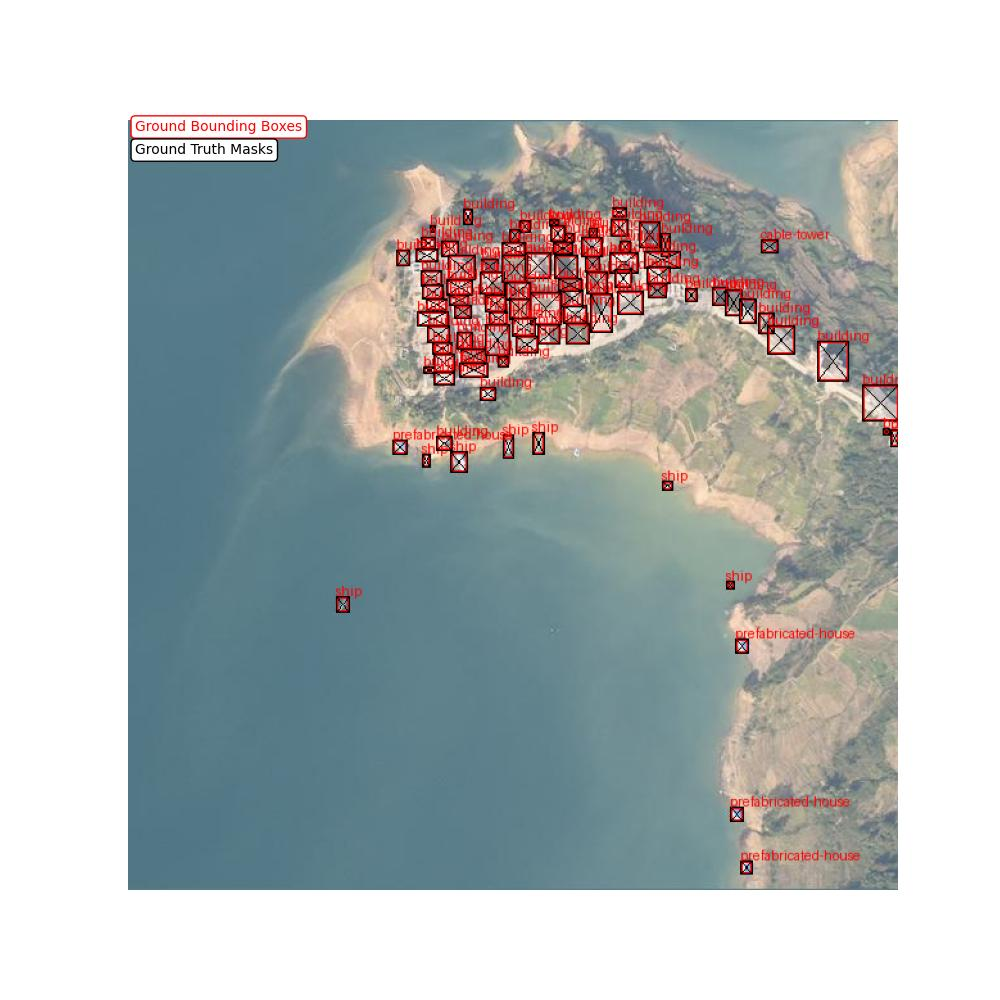
\includegraphics[scale=0.35]{Figures/uav_ground_truth.jpg}
      \caption{Ground Truth Bounding boxes and Masks}
    \end{minipage}
    \hfill
    \begin{minipage}{0.4\textwidth}
      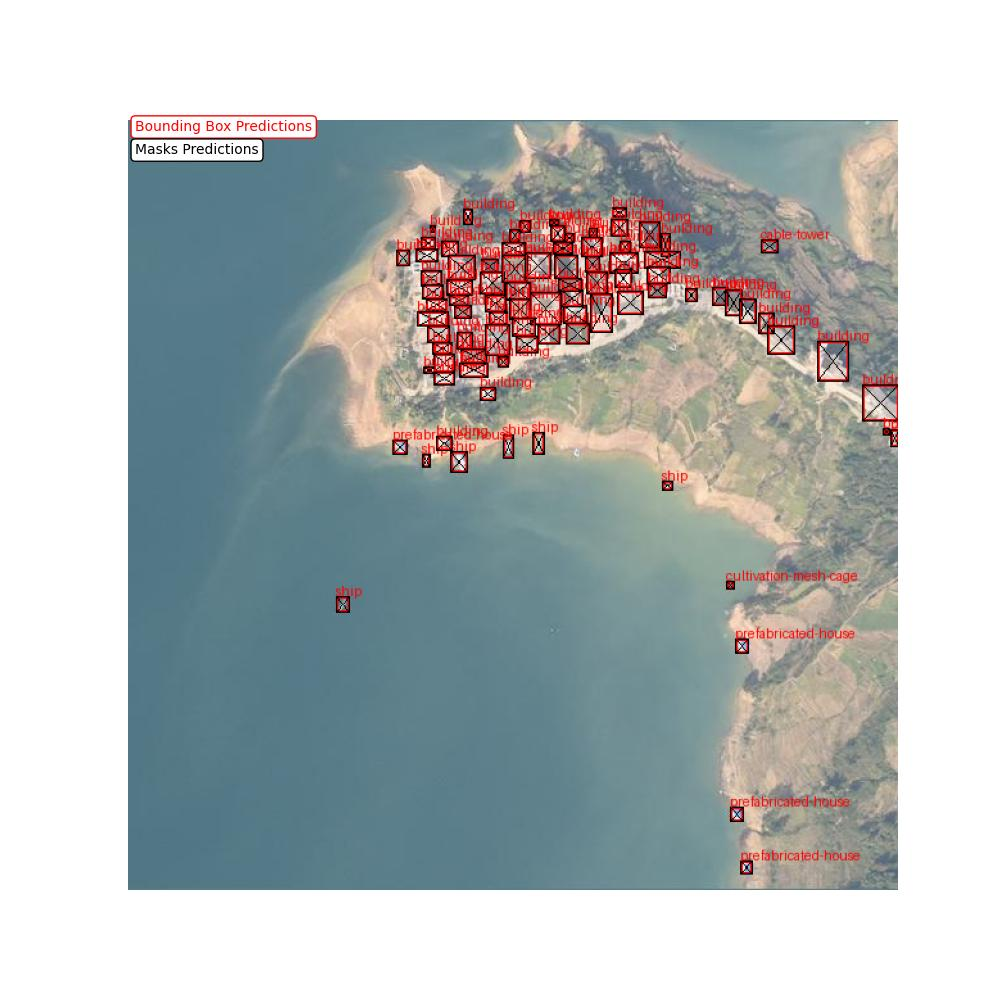
\includegraphics[scale=0.35]{Figures/uav_predictions.jpg}
      \caption{Predicted Bounding boxes and Masks}
    \end{minipage}
    \caption{Comparison between ground truth and predictions of EMAMT for the UAV-SOD dataset}
    \label{fig:uav-images}
\end{figure}


\subsection{VisDrone}

Similar to the UAV-SOD dataset, the proposed EMAMT model achieves a significant reduction in trainable parameters, being 56\% lighter than the original MAMT. 
However, in the VisDrone dataset, this comes at a noticeable performance trade-off, with a drop of around 13.7\% in mAP(@0.5) and 10\% in mAP(@0.5:0.95). Despite 
this reduction in performance, the lighter architecture of EMAMT offers benefits in terms of computational efficiency. As the table \ref{tab:vis_results} summarizes 
the performance of both models, showcasing the balance between model complexity and detection performance on small object datasets.


\begin{table}[h]
    \centering
    \begin{tabular}{|c|c|c|c|c|c|}
        \hline
        \textbf{Model}     & \textbf{mAP(@0.5)}     & \textbf{mAP(@0.5:0.95)}    & \textbf{Queries}   & \textbf{Parameters} & \textbf{GFLOPs}  \\ \hline
        EMAMT              & 39.5                   & 29.2                       & \textbf{100}       & \textbf{95M}        &  \textbf{492}     \\ \hline
        MAMT               & \textbf{53.2}          & \textbf{39.2}              & 200                & 216M                &  868              \\ \hline
    \end{tabular}
    \caption{Results for VisDrone dataset}
    \label{tab:vis_results}
\end{table}


Similarly both models exhibit a sharp rise in performance during the first 20 epochs, with MAMT clearly outperforming EMAMT throughout the training. In the 
mAP@0.5 plot, MAMT reaches a higher final performance of approximately 53\%, while EMAMT plateaus around 39\%. Similarly, for mAP@0.5:0.95, MAMT achieves 
around 39\%, while EMAMT settles at around 29\%.

These results highlight the stronger performance of MAMT over EMAMT for object detection in the VisDrone dataset, which contains small and challenging objects. 
Despite being a lighter model, EMAMT shows a notable performance, but the more complex MAMT model offers a better ability to handle the intricacies of the dataset, 
as seen by the significant gap in both metrics.

\begin{figure}[h!]
    \centering
    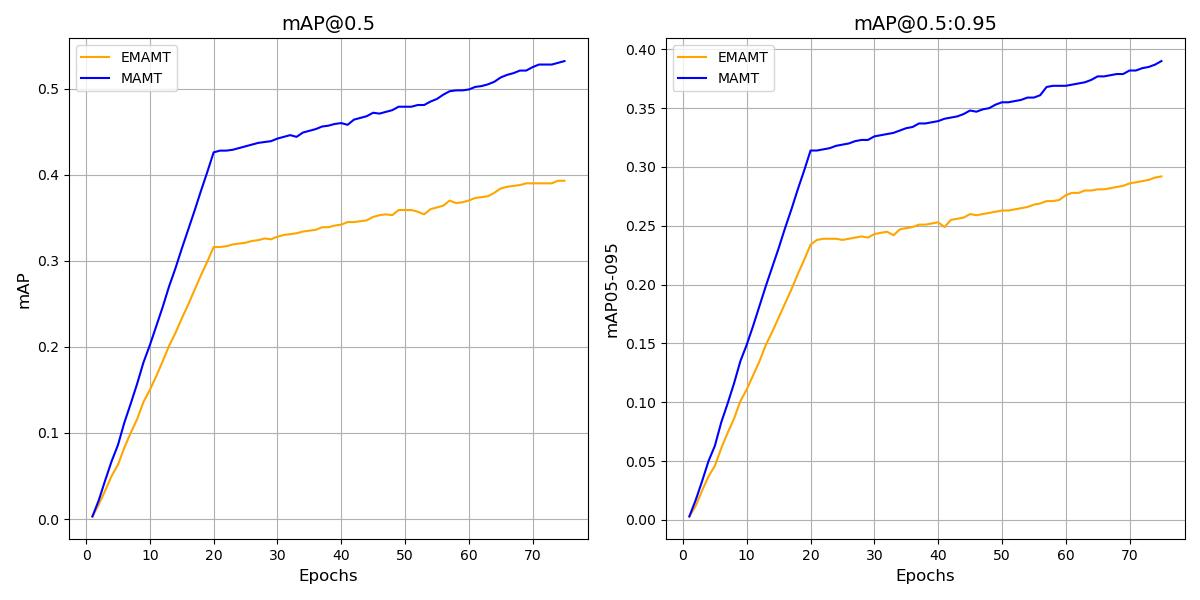
\includegraphics[scale=0.55]{Figures/vis_train.jpg}
    \caption{Performance comparison of MAMT and EMAMT on mAP at 50\% IoU threshold (left) and the average mAP across IoU thresholds from 50\% to 95\% (right) 
    for the VisDrone dataset}
    \label{fig:uav-train}
\end{figure}



As depicted in Figure \ref{fig:vis-images}, the model successfully detected most of the labelled objects. In this dataset we faced a variety of challenges including
a variable number size and quite a lot of missing annotations. This led to model detecting correctly many more objects than annotated by the dataset. These problems
can be found in both the train and validation set of the VisDrone dataset. 


\begin{figure}[!h]
    \captionsetup{justification=centering}
    \centering
    \begin{minipage}{0.4\textwidth}
      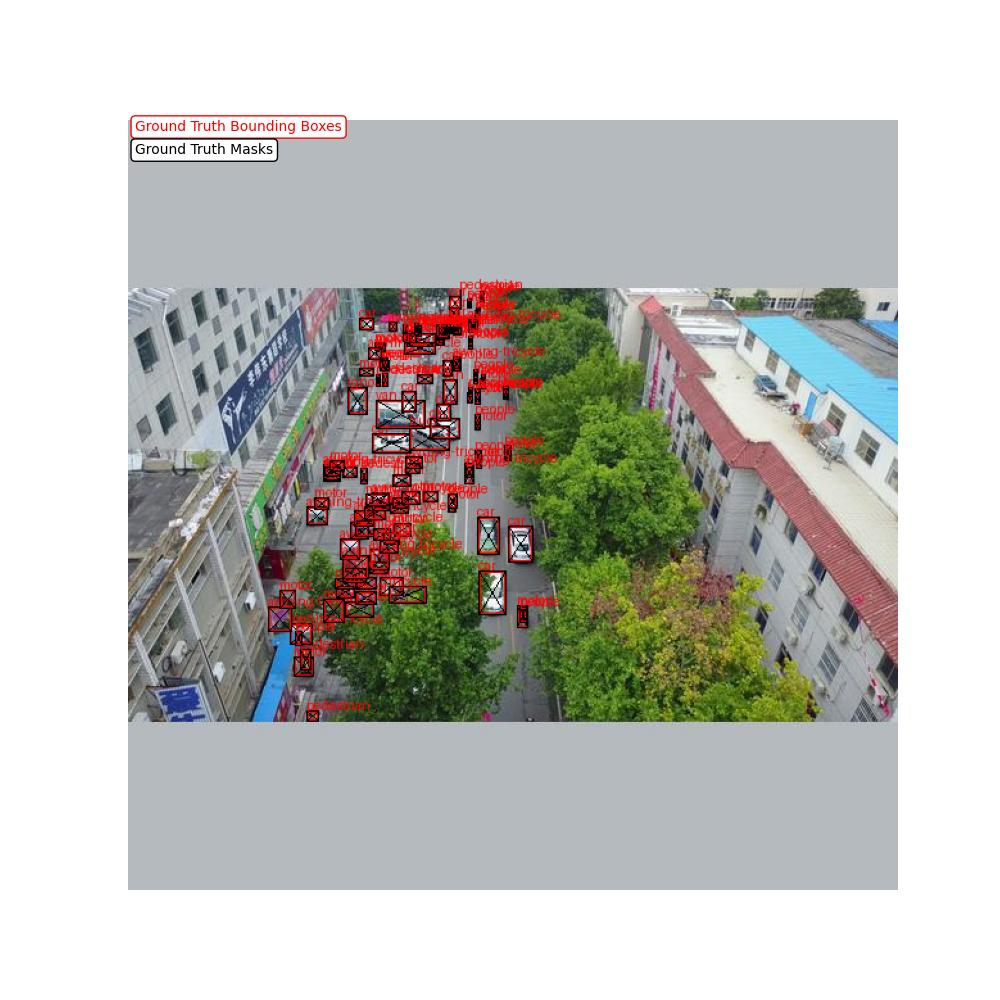
\includegraphics[scale=0.35]{Figures/vis_ground_truth.jpg}
      \caption{Ground Truth Bounding boxes and Masks}
    \end{minipage}
    \hfill
    \begin{minipage}{0.4\textwidth}
      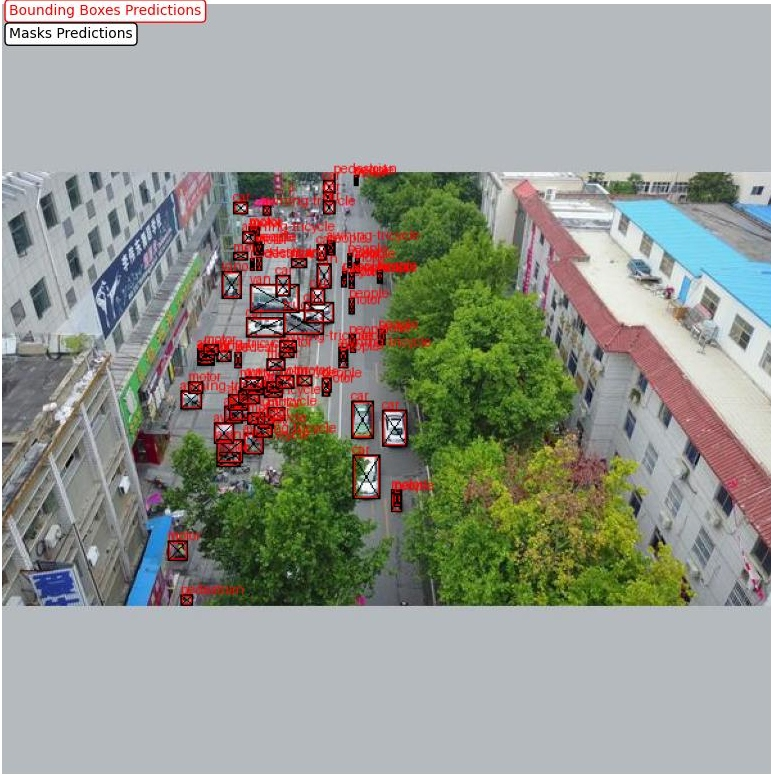
\includegraphics[scale=0.35]{Figures/vis_predictions.jpg}
      \caption{Predicted Bounding boxes and Masks}
    \end{minipage}
    \caption{Comparison between ground truth and predictions of EMAMT for the VisDrone dataset}
    \label{fig:vis-images}
\end{figure}


